% Interpolated correction at a held-out bearing (Study 1), in parts for content.tex:
%   Part 1 is two paragraphs for \subsection{Design} \label{sec:feas-s1-design},
%          after the production-session paragraph
%   Part 2 is a new subsection, placed after \subsection{Production Configuration}
%          \label{sec:results-s1-production} and before \subsection{Summary}
%   Part 3 (optional) is a sentence to append to the last paragraph of
%          \subsection{A Gain Correction, and Why It Does Not Hold} \label{sec:results-s1-validation}
% Requires: booktabs, pgfplots (compat=1.18), \abs from commands.tex. No siunitx.
% Numbers: python3 scripts/analyse_head_accuracy.py study/head_accuracy_production_cal2.csv --drop production_cal2:1 --moves
%          python3 scripts/analyse_head_accuracy.py study/head_accuracy_production_nocal2.csv --drop production_nocal2:1 --moves
%          The first also prints the calibration table. --drop leaves out trial 1 of each run (not analysed).
% Figure:  python3 scripts/analyse_head_accuracy.py study/head_accuracy_production_cal2.csv study/head_accuracy_production_nocal2.csv --drop production_cal2:1 production_nocal2:1 --pgf-until 4.5
% Table:   study/doa_angle_response_table125.csv, recorded with scripts/calibrate_doa_angles.py on 14 September 2026.

% ======================================================================
% Part 1 - method
% ======================================================================

A fourth session, on 14 September 2026, tested whether the angular response can
be corrected by interpolating between measured bearings where a single gain could
not (section~\ref{sec:results-s1-validation}). The response was first measured at
1.25\,m in quiet at 0, 30, 45, 75, 90, 135, 150 and 180\textdegree{}, three
repetitions each, using the script \texttt{calibrate\_doa\_angles.py}. The servo defined each
source position and the head returned home before the stimulus, as in the main
session; each repetition discarded the first 1.5\,s after the voice onset and took
the circular median of seven readings 250\,ms apart, and each point of the table
is the median of its three repetitions. 60\textdegree{} was left out, so that the
bearing at which the single gain failed was again held out, and 75\textdegree{} was
included so that 60\textdegree{} lies midway between two measured points rather
than inside the 45\textdegree{} gap between 45\textdegree{} and 90\textdegree{}.
With \texttt{DOA\_CALIBRATION\_PATH} set, the assistant maps every reading through
the table by linear interpolation, including readings taken after the head has
turned.

The source was then placed at 60\textdegree{} and 1.25\,m, verified by protractor,
and left in place for two runs in the production configuration of
section~\ref{sec:results-s1-production}: first with the table, then without it,
five trials each. The configuration
recorded with every trial confirms that the table was loaded with all eight points
in the first run and absent in the second.

% ======================================================================
% Part 2 - results
% ======================================================================

\subsection{An Interpolated Correction}
\label{sec:results-s1-table}

Table~\ref{tab:s1-table-points} lists the measured response. It is not a
compression by one factor: the bearings at 45\textdegree{} and 75\textdegree{} were
reported closer to the front than they are, those at 135\textdegree{} and
150\textdegree{} almost where they are, and the bearing at 30\textdegree{} further
from the front than it is.

\begin{table}[htb]
  \centering
  \caption{Angular response at 1.25\,m in quiet, used as the correction table:
  median reported bearing of three repetitions at each true bearing.
  60\textdegree{} was held out.}
  \label{tab:s1-table-points}
  \begin{tabular}{@{}lrrrrrrrr@{}}
    \toprule
    True (\textdegree)     & 0 & 30 & 45 & 75 & 90 & 135 & 150 & 180 \\
    Reported (\textdegree) & 0 & 25 & 50 & 79 & 90 & 133 & 149 & 180 \\
    \bottomrule
  \end{tabular}
\end{table}

Table~\ref{tab:s1-table-60} compares the two runs at 60\textdegree{}, and
figure~\ref{fig:s1-table-60} shows every trial over time. Neither run had a
detection failure.

\begin{table}[htb]
  \centering
  \small
  \caption{Production configuration at 60\textdegree{}, 1.25\,m, quiet, five trials
  per run. Errors are commanded heading minus true bearing; times are median [IQR]
  from the array's first voice report. \emph{Last turn} is the last servo update
  that changed the heading; \emph{latency} is the measure of
  section~\ref{sec:results-s1-latency}, which also counts estimates that left the
  head where it was.}
  \label{tab:s1-table-60}
  \begin{tabular}{@{}lll@{}}
    \toprule
    & Without table & With table \\
    \midrule
    Median $\abs{e}$ after the first move (\textdegree) & 7.00 & 0.52 \\
    Median $\abs{e}$, final (\textdegree)               & 2.00 [1.00, 2.00] & 0.52 [0.52, 1.55] \\
    Signed $e$, final, mean $\pm$ SD (\textdegree)      & $+0.80 \pm 1.92$ & $-1.32 \pm 1.94$ \\
    Largest $\abs{e}$, final (\textdegree)              & 3.00 & 4.54 \\
    Trials in which the head turned after the first move & 5/5 & 1/5 \\
    \addlinespace
    First move complete (s) & 0.474 [0.446, 0.482] & 0.514 [0.514, 0.518] \\
    Last turn complete (s)  & 1.483 [1.481, 1.493] & 0.518 [0.514, 0.547] \\
    Latency (s)             & 1.483 [1.481, 1.493] & 1.394 [1.394, 1.410] \\
    \bottomrule
  \end{tabular}
\end{table}

Without the table, the head behaved as at 45\textdegree{} and 135\textdegree{} in
the production session. The first move stopped short, a median 7.00\textdegree{}
from the source, and a second estimate, taken with the source close to the head's
axis, turned it again in all five trials, to a final median error of
2.00\textdegree{} (IQR 1.00--2.00\textdegree{}). The last turn was complete a
median 1.483\,s after the first voice report.

With the table, the first move was complete after a median 0.514\,s and left the
head a median 0.52\textdegree{} from the source. In four of the five trials it was
the only turn: where a further estimate followed, it came out at 90\textdegree{}
and left the head in place. The final median error was 0.52\textdegree{} (IQR
0.52--1.55\textdegree{}), and the last turn was complete a median 0.518\,s after
the first voice report. The latency measure gives 1.394\,s for this run only
because it also counts those further estimates.

\begin{figure}[htb]
  \centering
  \definecolor{nocalc}{HTML}{9A9A9A}
  \definecolor{calc}{HTML}{EB6834}
  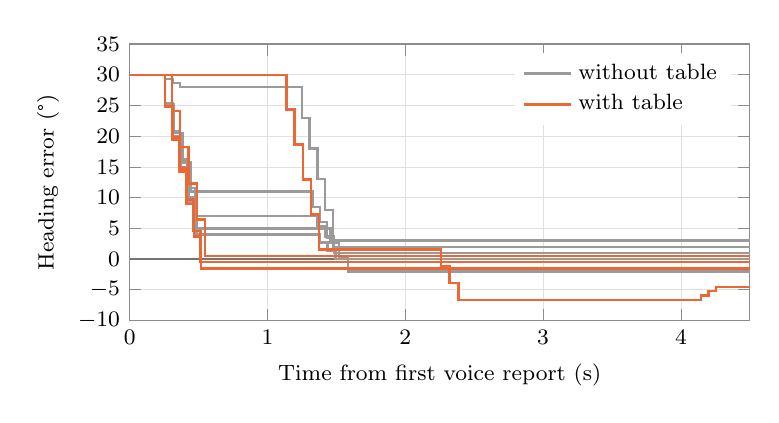
\begin{tikzpicture}
    \begin{axis}[
      width=0.78\textwidth, height=0.42\textwidth,
      xmin=0, xmax=4.5, xtick={0,1,2,3,4},
      ymin=-10, ymax=35, ytick={-10,-5,0,5,10,15,20,25,30,35},
      xlabel={Time from first voice report (s)},
      ylabel={Heading error (\textdegree)},
      tick label style={font=\footnotesize},
      label style={font=\footnotesize},
      grid=major, grid style={line width=0.2pt, draw=black!12},
      axis line style={draw=black!45}, tick style={draw=black!45},
      legend style={at={(0.97,0.97)}, anchor=north east, font=\footnotesize,
                    draw=none, fill=white, cells={anchor=west}},
    ]
      \addplot[black!55, line width=0.6pt, domain=0:4.5, samples=2, forget plot] {0};
      % production_nocal2 trial 2
      \addplot[nocalc, line width=0.9pt]
        coordinates {(0.000,30.00) (0.258,30.00) (0.258,25.25) (0.321,25.25) (0.321,20.50) (0.383,20.50) (0.383,15.75) (0.445,15.75) (0.445,11.00) (1.330,11.00) (1.330,8.50) (1.381,8.50) (1.381,6.00) (1.432,6.00) (1.432,3.50) (1.483,3.50) (1.483,1.00) (4.500,1.00)};
      \addlegendentry{without table}
      % production_nocal2 trial 3
      \addplot[nocalc, line width=0.9pt, forget plot]
        coordinates {(0.000,30.00) (0.258,30.00) (0.258,25.00) (0.314,25.00) (0.314,20.00) (0.370,20.00) (0.370,15.00) (0.426,15.00) (0.426,10.00) (0.482,10.00) (0.482,5.00) (1.458,5.00) (1.458,2.67) (1.521,2.67) (1.521,0.33) (1.583,0.33) (1.583,-2.00) (4.500,-2.00)};
      % production_nocal2 trial 4
      \addplot[nocalc, line width=0.9pt, forget plot]
        coordinates {(0.000,30.00) (0.258,30.00) (0.258,29.33) (0.313,29.33) (0.313,28.67) (0.367,28.67) (0.367,28.00) (1.250,28.00) (1.250,23.00) (1.306,23.00) (1.306,18.00) (1.362,18.00) (1.362,13.00) (1.418,13.00) (1.418,8.00) (1.474,8.00) (1.474,3.00) (4.500,3.00)};
      % production_nocal2 trial 5
      \addplot[nocalc, line width=0.9pt, forget plot]
        coordinates {(0.000,30.00) (0.258,30.00) (0.258,24.80) (0.315,24.80) (0.315,19.60) (0.372,19.60) (0.372,14.40) (0.429,14.40) (0.429,9.20) (0.486,9.20) (0.486,4.00) (1.378,4.00) (1.378,2.67) (1.436,2.67) (1.436,1.33) (1.493,1.33) (1.493,0.00) (4.500,0.00)};
      % production_nocal2 trial 6
      \addplot[nocalc, line width=0.9pt, forget plot]
        coordinates {(0.000,30.00) (0.258,30.00) (0.258,25.40) (0.312,25.40) (0.312,20.80) (0.366,20.80) (0.366,16.20) (0.420,16.20) (0.420,11.60) (0.474,11.60) (0.474,7.00) (1.362,7.00) (1.362,5.33) (1.421,5.33) (1.421,3.67) (1.481,3.67) (1.481,2.00) (4.500,2.00)};
      % production_cal2 trial 2
      \addplot[calc, line width=0.9pt]
        coordinates {(0.000,30.00) (0.258,30.00) (0.258,24.91) (0.310,24.91) (0.310,19.83) (0.361,19.83) (0.361,14.74) (0.412,14.74) (0.412,9.66) (0.463,9.66) (0.463,4.57) (0.514,4.57) (0.514,-0.52) (4.500,-0.52)};
      \addlegendentry{with table}
      % production_cal2 trial 3
      \addplot[calc, line width=0.9pt, forget plot]
        coordinates {(0.000,30.00) (0.258,30.00) (0.258,24.74) (0.310,24.74) (0.310,19.48) (0.362,19.48) (0.362,14.22) (0.414,14.22) (0.414,8.97) (0.466,8.97) (0.466,3.71) (0.518,3.71) (0.518,-1.55) (4.500,-1.55)};
      % production_cal2 trial 4
      \addplot[calc, line width=0.9pt, forget plot]
        coordinates {(0.000,30.00) (0.306,30.00) (0.306,24.10) (0.366,24.10) (0.366,18.21) (0.426,18.21) (0.426,12.31) (0.487,12.31) (0.487,6.41) (0.547,6.41) (0.547,0.52) (4.500,0.52)};
      % production_cal2 trial 5
      \addplot[calc, line width=0.9pt, forget plot]
        coordinates {(0.000,30.00) (1.138,30.00) (1.138,24.31) (1.197,24.31) (1.197,18.62) (1.257,18.62) (1.257,12.93) (1.316,12.93) (1.316,7.24) (1.375,7.24) (1.375,1.55) (2.258,1.55) (2.258,-1.18) (2.322,-1.18) (2.322,-3.90) (2.387,-3.90) (2.387,-6.63) (4.146,-6.63) (4.146,-5.93) (4.200,-5.93) (4.200,-5.23) (4.254,-5.23) (4.254,-4.54) (4.500,-4.54)};
      % production_cal2 trial 6
      \addplot[calc, line width=0.9pt, forget plot]
        coordinates {(0.000,30.00) (0.258,30.00) (0.258,24.91) (0.309,24.91) (0.309,19.83) (0.361,19.83) (0.361,14.74) (0.412,14.74) (0.412,9.66) (0.463,9.66) (0.463,4.57) (0.514,4.57) (0.514,-0.52) (4.500,-0.52)};
    \end{axis}
  \end{tikzpicture}
  \caption{Heading error (commanded heading minus true bearing) over time at
  60\textdegree{}, 1.25\,m, quiet, in the production configuration, one line per
  trial, stepped at every servo update and held after the last. The head starts at
  home, 30\textdegree{} from the source. Grey: without the table; orange: with it.
  The orange line that turns late and dips below zero is trial~5.}
  \label{fig:s1-table-60}
\end{figure}

The one exception with the table, trial~5, shows two ways the correction can still
miss. Four of the five readings behind its first estimate still pointed straight
ahead, so the head did not turn until the second estimate, which took it to
61.55\textdegree{}. An estimate taken with the head there, almost facing the
source, came out at 81.82\textdegree{} after mapping and turned the head to
53.37\textdegree{}; the last of five estimates left it at 55.46\textdegree{},
4.54\textdegree{} past the source. The table acts on such near-axis readings as
much as on the first: it maps the 11\textdegree{} between reported 79\textdegree{}
and 90\textdegree{} onto the 15\textdegree{} between true 75\textdegree{} and
90\textdegree{}, so a small error close to the head's axis is enlarged rather than
reduced.

The comparison with the single-gain correction of
section~\ref{sec:results-s1-validation} is closest for the first move, since both
rest on one estimate taken with the head at home. With the gain, the error at
60\textdegree{} was $+6.87$\textdegree{}; with the table, the first move was a
median 0.52\textdegree{} from the source, and without any correction
7.00\textdegree{}. The two are not measured identically. The validation session
used the study configuration, which waits 1.5\,s and then samples for a further
second, whereas these runs sample at the onset, and the gain result is computed
from a session mean of signed error whereas the figures here are medians of
absolute error. Within those limits, interpolating between measured bearings
generalised to the held-out bearing where the single constant did not.

The result does not reach further than that. The table was measured in the same
room, at the same distance and on the same day as the runs it corrected, and it was
tested at one bearing, in quiet, with five trials per run. At that bearing the
production configuration came within 3.00\textdegree{} of the source without any
correction, because its second estimate is taken close to the head's axis. What
the table added there is that the head reached its final bearing on the first
move, after 0.518\,s instead of 1.483\,s, rather than a clearly more accurate final
bearing: the final errors of the two runs overlap. Whether the table holds at other
distances or under babble, where the response itself differs
(sections~\ref{sec:results-s1-distance} and~\ref{sec:results-s1-noise}), was not
tested.

% ======================================================================
% Part 3 (optional) - append to the last paragraph of
% \subsection{A Gain Correction, and Why It Does Not Hold}, after
% "... sampled across the arc and interpolated."
% ======================================================================

% Section~\ref{sec:results-s1-table} tests such a correction at the same held-out
% bearing.
